\chapter{PROPOSED SYSTEM AND METHODOLOGY}

\section{SYSTEM ARCHITECTURE}
The architecture of the proposed machine learning system is engineered to provide an automated, leak-free, reproducible pipeline spanning raw data ingestion, statistical auditing, stratified splitting, preprocessing, supervised classification, feature attribution, unsupervised customer segmentation, and strategic retention decision support. Figure~\ref{fig:system_arch} illustrates the complete end-to-end operational architecture.

\begin{figure}[H]
    \centering
    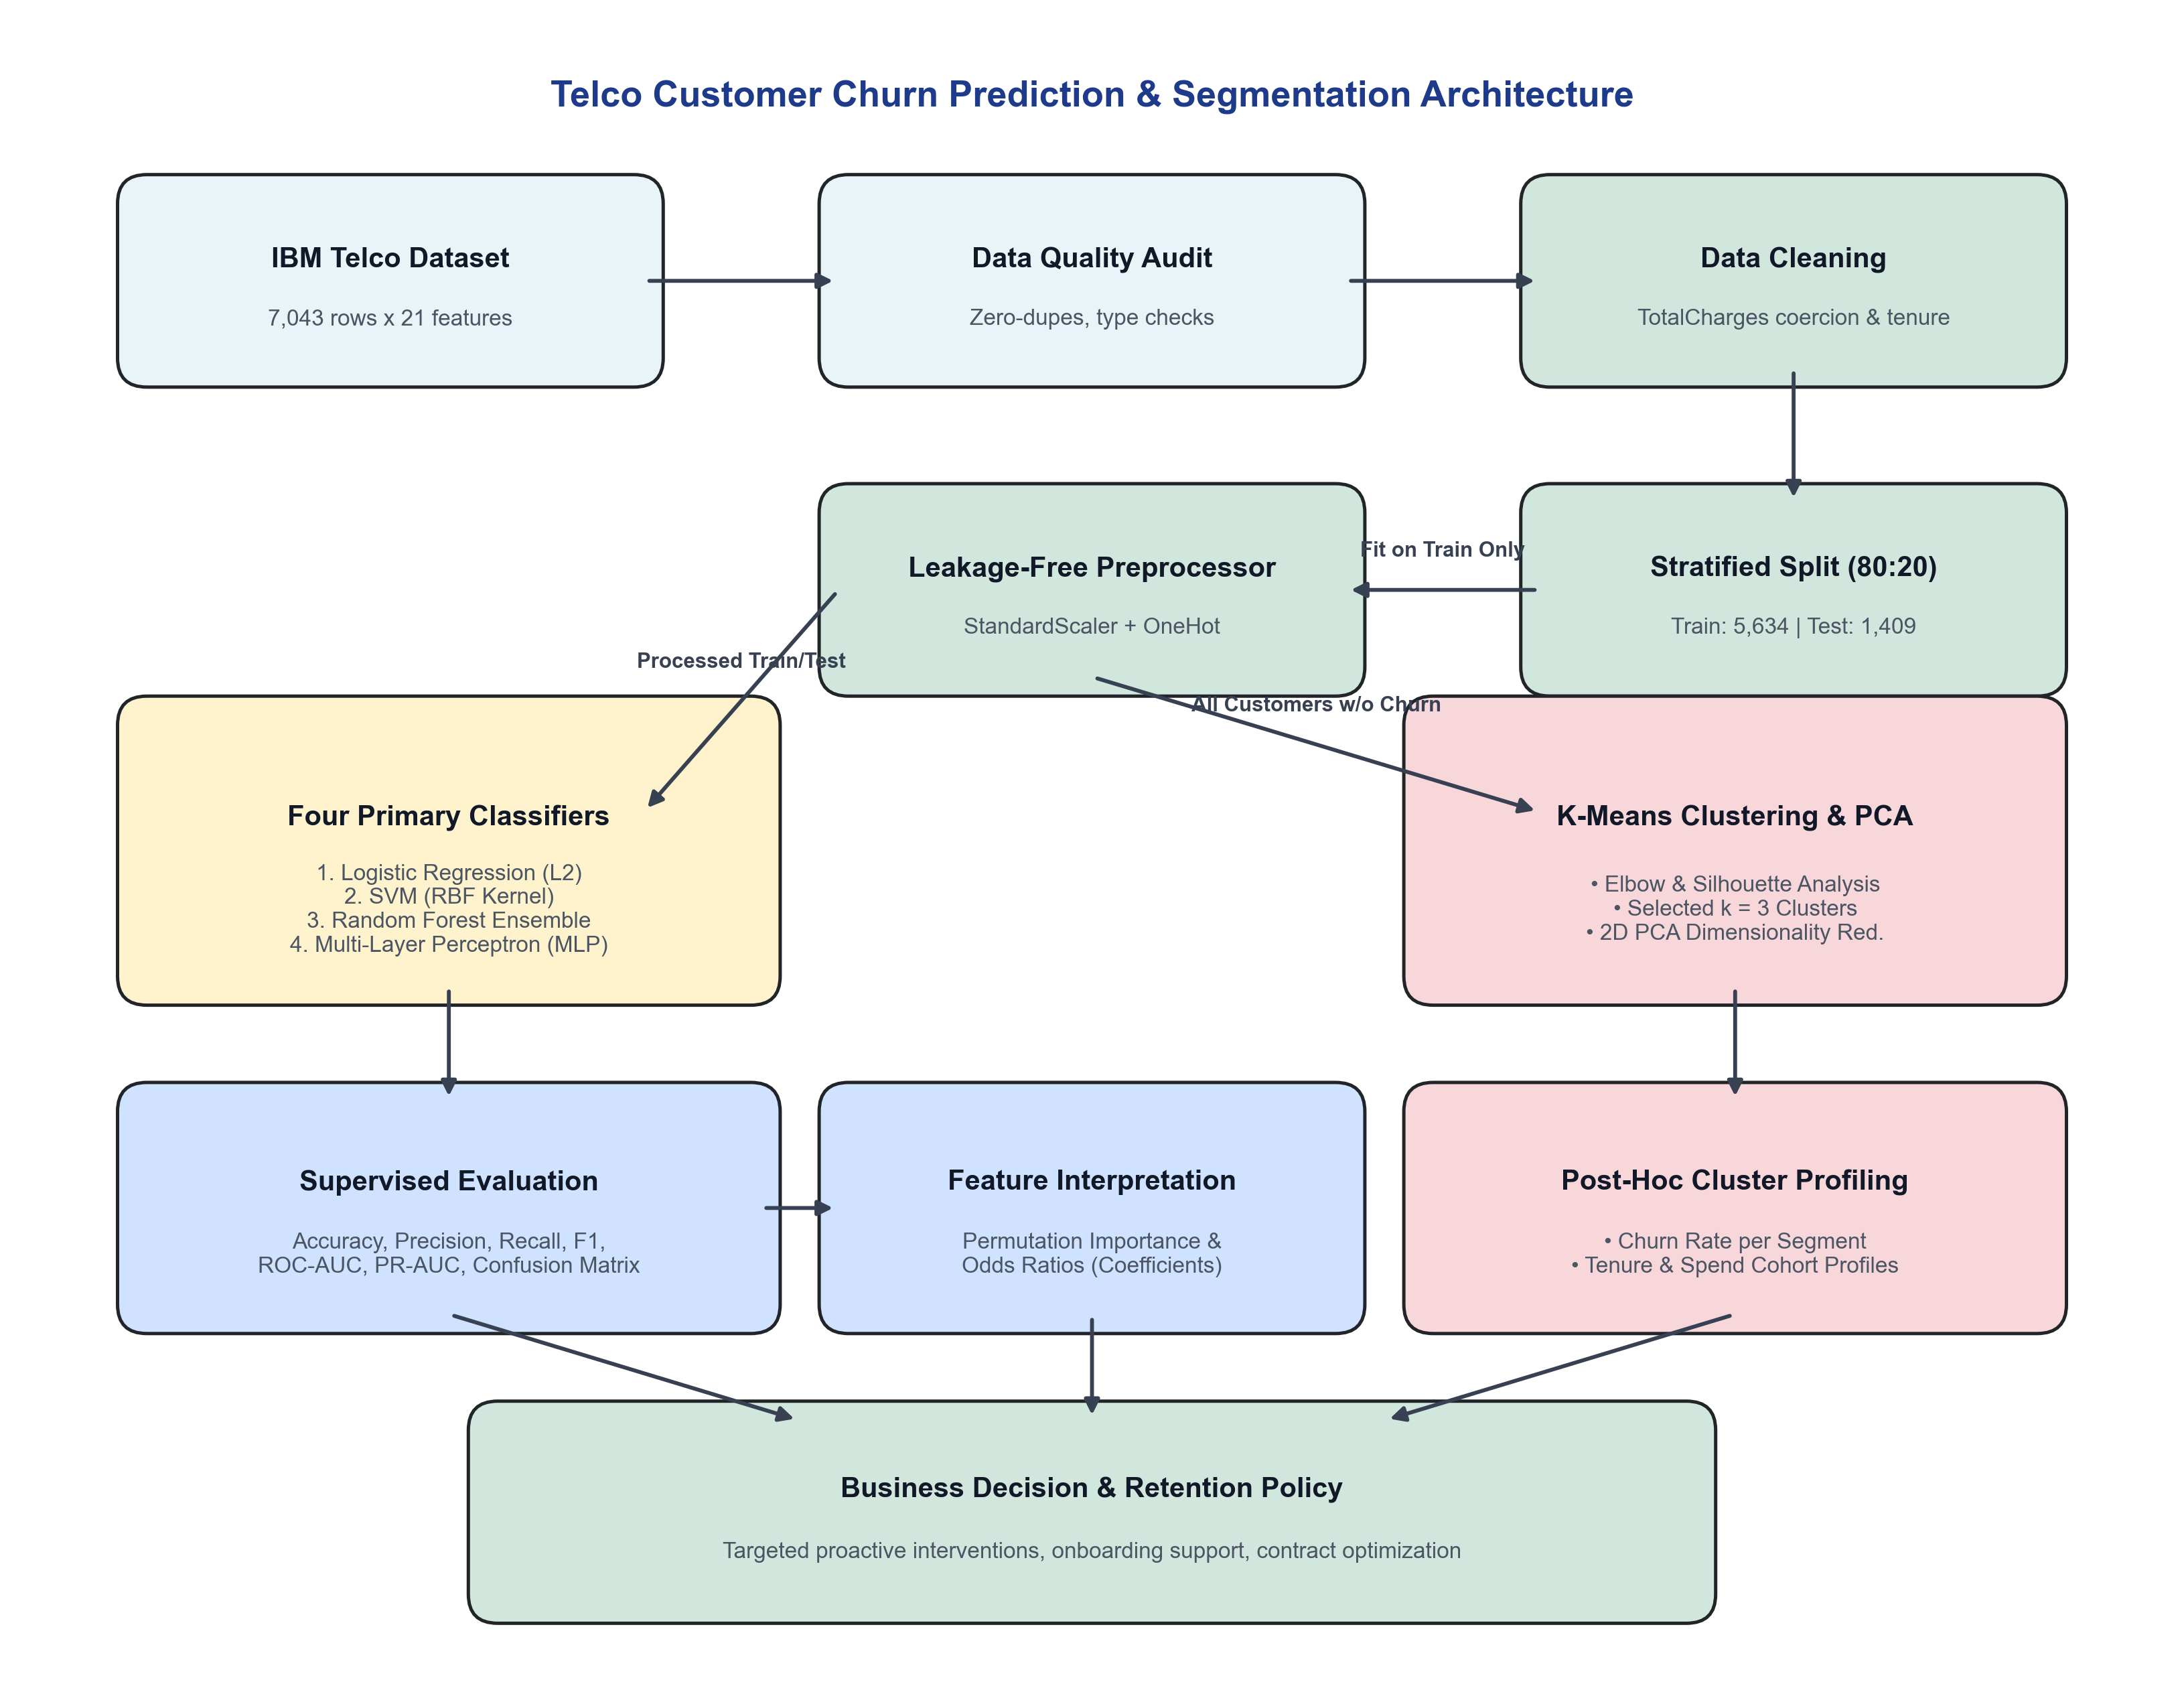
\includegraphics[width=0.95\textwidth]{figures/system_architecture.png}
    \caption{End-to-End System Architecture for Churn Prediction and Customer Segmentation}
    \label{fig:system_arch}
\end{figure}

The pipeline operates in six strictly decoupled sequential stages:
\begin{enumerate}
    \item \textbf{Data Ingestion \& Validation Layer:} Ingests the benchmark IBM Telco dataset, validates row/column counts (\datasetTotalRows{} rows, \datasetTotalCols{} features), checks for record duplicates, and audits data types.
    \item \textbf{Data Cleaning \& Leakage-Free Stratified Split:} Safely coerces \texttt{TotalCharges} to floating-point numbers, maps target \texttt{Churn} to binary integers (0/1), preserves \texttt{customerID} as an external tracking index, and executes an 80:20 stratified split into training (\datasetTrainCount{} rows) and test (\datasetTestCount{} rows) subsets.
    \item \textbf{Isolated Preprocessing Transformers:} Constructs a scikit-learn \texttt{ColumnTransformer} featuring median imputation and standard scaling for numerical features alongside most-frequent imputation and one-hot encoding for categorical attributes. Crucially, this transformer is fitted strictly on the training set.
    \item \textbf{Supervised Comparative Classification Layer:} Concurrently trains and evaluates four primary classifiers (Logistic Regression, Support Vector Machine, Random Forest, and Multi-Layer Perceptron) using balanced class weighting and 5-fold training cross-validation.
    \item \textbf{Feature Attribution \& Model Interpretation:} Executes permutation importance on the uncorrupted held-out test set to isolate predictive variables, accompanied by log-odds coefficient extraction.
    \item \textbf{Unsupervised Segmentation \& Post-Hoc Analysis:} Evaluates K-Means cluster candidates across $k \in [2, 8]$ using Elbow and Silhouette analysis, projects clusters into 2D via PCA, and links target churn rates post-hoc to generate differentiated retention strategies.
\end{enumerate}

\section{DATASET DESCRIPTION}
The empirical investigation utilizes the public IBM Telco Customer Churn benchmark dataset \citep{ibm2019telco}. The dataset comprises \datasetTotalRows{} customer records, with each record documented across 21 distinct variables spanning four operational categories:
\begin{itemize}
    \item \textbf{Customer Demographics:}
    \begin{itemize}
        \item \texttt{customerID}: Unique alphanumeric customer identifier (excluded from predictive feature matrices).
        \item \texttt{gender}: Customer biological sex (Male, Female).
        \item \texttt{SeniorCitizen}: Binary demographic indicator (1 for senior citizen, 0 otherwise).
        \item \texttt{Partner}: Whether customer has a domestic partner (Yes, No).
        \item \texttt{Dependents}: Whether customer resides with financial dependents (Yes, No).
    \end{itemize}
    \item \textbf{Subscribed Services:}
    \begin{itemize}
        \item \texttt{tenure}: Total continuous duration of customer subscription in months (integer, range: 0--72).
        \item \texttt{PhoneService}: Whether customer subscribes to fixed landline telephone service (Yes, No).
        \item \texttt{MultipleLines}: Whether customer utilizes multiple telephone connections (Yes, No, No phone service).
        \item \texttt{InternetService}: Core broadband technology provider (DSL, Fiber optic, No).
        \item \texttt{OnlineSecurity}: Value-added internet security service (Yes, No, No internet service).
        \item \texttt{OnlineBackup}: Cloud-based offsite storage backup service (Yes, No, No internet service).
        \item \texttt{DeviceProtection}: Hardware insurance and device warranty plan (Yes, No, No internet service).
        \item \texttt{TechSupport}: Priority technical assistance plan (Yes, No, No internet service).
        \item \texttt{StreamingTV}: Streaming television digital television service (Yes, No, No internet service).
        \item \texttt{StreamingMovies}: Streaming digital cinema and video-on-demand service (Yes, No, No internet service).
    \end{itemize}
    \item \textbf{Contractual and Account Information:}
    \begin{itemize}
        \item \texttt{Contract}: Subscription contract duration commitment (Month-to-month, One year, Two year).
        \item \texttt{PaperlessBilling}: Whether customer receives invoices electronically (Yes, No).
        \item \texttt{PaymentMethod}: Customer billing settlement mechanism (Electronic check, Mailed check, Bank transfer (automatic), Credit card (automatic)).
        \item \texttt{MonthlyCharges}: Customer current monthly subscription billing amount in US dollars (continuous float).
        \item \texttt{TotalCharges}: Cumulative lifetime billing billed to customer in US dollars (continuous float).
    \end{itemize}
    \item \textbf{Ground-Truth Target:}
    \begin{itemize}
        \item \texttt{Churn}: Whether customer discontinued service within the last recorded month (Yes: \datasetChurnProportion{}, No: \datasetRetainedProportion{}).
    \end{itemize}
\end{itemize}

\section{DATA PRE-PROCESSING}
To guarantee mathematical rigor and prevent data leakage, preprocessing steps are strictly sequenced as follows:
\begin{itemize}
    \item \textbf{Type Coercion and Whitespace Elimination:} In the raw CSV, \texttt{TotalCharges} contains 11 instances of blank whitespace strings (\texttt{" "}). Inspection of these records confirms that all 11 instances correspond exactly to newly enrolled subscribers with $\texttt{tenure} = 0$. These empty values are safely coerced to \texttt{NaN} and assigned the exact domain-valid value of \texttt{0.0}, reflecting zero prior billing cycles.
    \item \textbf{Target Encoding and Identifier Isolation:} The binary target \texttt{Churn} is mapped to $y \in \{0, 1\}$ (\texttt{No} $\to 0$, \texttt{Yes} $\to 1$). \texttt{customerID} is removed from the predictor matrix $\mathbf{X}$ to eliminate spurious high-cardinality memorization.
    \item \textbf{Stratified Splitting:} The dataset is partitioned into an 80\% training split ($N=\datasetTrainCount{}$) and a 20\% test split ($N=\datasetTestCount{}$) using stratified sampling on $y$ with fixed seed $\texttt{random\_state}=42$. This guarantees that both partitions mirror the true population churn prevalence ($\approx 26.54\%$).
    \item \textbf{Numerical Pipeline (Standardization):} For numerical features (\texttt{tenure}, \texttt{MonthlyCharges}, \texttt{TotalCharges}), a pipeline consisting of a \texttt{SimpleImputer(strategy='median')} followed by \texttt{StandardScaler} is fitted exclusively on $\mathbf{X}_{\text{train}}$:
    \begin{equation}
        z = \frac{x - \mu_{\text{train}}}{\sigma_{\text{train}}}
    \end{equation}
    The learned training parameters ($\mu_{\text{train}}, \sigma_{\text{train}}$) are subsequently applied to scale $\mathbf{X}_{\text{test}}$.
    \item \textbf{Categorical Pipeline (One-Hot Encoding):} The 16 categorical predictors are processed through \texttt{OneHotEncoder(handle\_unknown='ignore', sparse\_output=False)}. This transforms the categorical space into 43 indicator features, yielding a final transformed feature space of $d=46$ dimensions.
\end{itemize}

\section{FEATURE ANALYSIS}
Feature analysis investigates the empirical relationships between customer attributes and attrition. In telecommunications, customer retention is governed by customer tenure dynamics, price elasticity, and commitment contracts. In Chapter~\ref{ch:results}, we employ exploratory visualizations alongside permutation feature importance on the held-out test set to isolate which factors legitimately account for model decision-making.

\section{MODEL BUILDING}
To provide a fair, balanced, and comprehensive comparison, exactly four primary classification algorithms are implemented:
\begin{itemize}
    \item \textbf{Model 1: Logistic Regression (L2 Baseline):}
    Provides an interpretable linear probabilistic baseline. Configured with an L2 ridge penalty ($C=1.0$), L-BFGS optimization solver, balanced class weighting to counter the $73.5:26.5$ negative-to-positive ratio, and maximum 1,000 iterations.
    
    \item \textbf{Model 2: Support Vector Machine (RBF Kernel):}
    Evaluates nonlinear margin-based discrimination in an infinite-dimensional RKHS. Configured with a Radial Basis Function kernel, scaling parameter $\gamma = 1 / (d \cdot \text{Var}(X))$, penalty parameter $C=1.0$, balanced class weighting, and Platt probability scaling for ROC/PR thresholding.
    
    \item \textbf{Model 3: Random Forest Classifier (Ensemble Bagging):}
    Evaluates ensemble bagging across 150 shallow randomized decision trees (\texttt{max\_depth=10}, \texttt{min\_samples\_split=5}, \texttt{min\_samples\_leaf=2}). Balanced class weighting is integrated into individual tree bootstrap subsamples to counter class imbalance natively.
    
    \item \textbf{Model 4: Multi-Layer Perceptron (Artificial Neural Network):}
    Demonstrates nonlinear representation learning via a fully connected feedforward architecture with two hidden layers: Layer 1 (64 units, ReLU) and Layer 2 (32 units, ReLU). Optimized using the Adam algorithm with learning rate $\eta=0.001$, mini-batch size 64, L2 weight regularization $\alpha=0.01$, and early stopping with patience of 15 iterations.
\end{itemize}

\section{EVALUATION METRICS}
To evaluate model performance objectively on the held-out test set, the following metrics are computed:
\begin{itemize}
    \item \textbf{Accuracy:} The proportion of total correct predictions: $\frac{\text{TP} + \text{TN}}{\text{TP} + \text{TN} + \text{FP} + \text{FN}}$.
    \item \textbf{Precision:} The proportion of flagged customers who actually churn: $\frac{\text{TP}}{\text{TP} + \text{FP}}$.
    \item \textbf{Recall (Sensitivity):} The proportion of actual churners successfully identified: $\frac{\text{TP}}{\text{TP} + \text{FN}}$.
    \item \textbf{F1-Score:} The harmonic mean of Precision and Recall: $2 \cdot \frac{\text{Precision} \cdot \text{Recall}}{\text{Precision} + \text{Recall}}$.
    \item \textbf{Specificity:} The True Negative Rate: $\frac{\text{TN}}{\text{TN} + \text{FP}}$.
    \item \textbf{Balanced Accuracy:} The arithmetic mean of Recall and Specificity: $\frac{\text{Recall} + \text{Specificity}}{2}$.
    \item \textbf{ROC-AUC:} Area under the True Positive Rate vs. False Positive Rate curve across all thresholds.
    \item \textbf{PR-AUC (Average Precision):} Area under the Precision-Recall curve, providing a rigorous metric under positive-class sparsity.
    \item \textbf{Training Time:} Total wall-clock time in seconds consumed during model fitting and hyperparameter optimization.
\end{itemize}

\section{TOOLS AND TECHNOLOGIES}
The implementation is constructed using a modern, reproducible Python 3 open-source stack:
\begin{itemize}
    \item \textbf{Python (v3.13):} High-performance programming language powering the core workflow.
    \item \textbf{pandas (v3.0.5) \& NumPy (v2.3.4):} High-throughput tabular data structures and multidimensional array vectorization.
    \item \textbf{scikit-learn (v1.9.0):} Industry-standard machine learning library providing the pipelines, transformers, classification models, cross-validation engines, and evaluation metrics.
    \item \textbf{Matplotlib (v3.10.7) \& Seaborn (v0.13.2):} Publication-grade plotting engines configured with the headless Agg backend for automated 300 DPI vector-like graphic synthesis.
    \item \textbf{Joblib (v1.5.2):} Lightweight object serialization for saving trained model pipelines and transformers.
    \item \textbf{pytest (v9.1.1):} Automated unit testing framework validating pipeline integrity and assertions.
    \item \textbf{MiKTeX pdfTeX (v4.23):} Academic typesetting engine compiling the final formal case study report.
\end{itemize}
